\clearpage

\section{M-QAM Receiver}\label{lib:homodyneRx}

\begin{tcolorbox}	
	\begin{tabular}{p{2.75cm} p{0.2cm} p{10.5cm}} 	
		\textbf{Header File}   &:& m\_qam\_receiver.h \\
		\textbf{Source File}   &:& m\_qam\_receiver.cpp \\
        \textbf{Version}       &:& 20180815 (\emph{Pedro Loureiro})\\
	\end{tabular}
\end{tcolorbox}

This block simulates the reception and demodulation of an optical
signal (which is the input signal of the system) and outputs a binary signal
corresponding to the reconstructed transmitted bitstream, which will later be used to calculate bit error rate (BER).
 A simplified schematic representation of this block is shown in figure
\ref{fig:homodyneRx_simple}.
\begin{figure}[H]
	\centering
	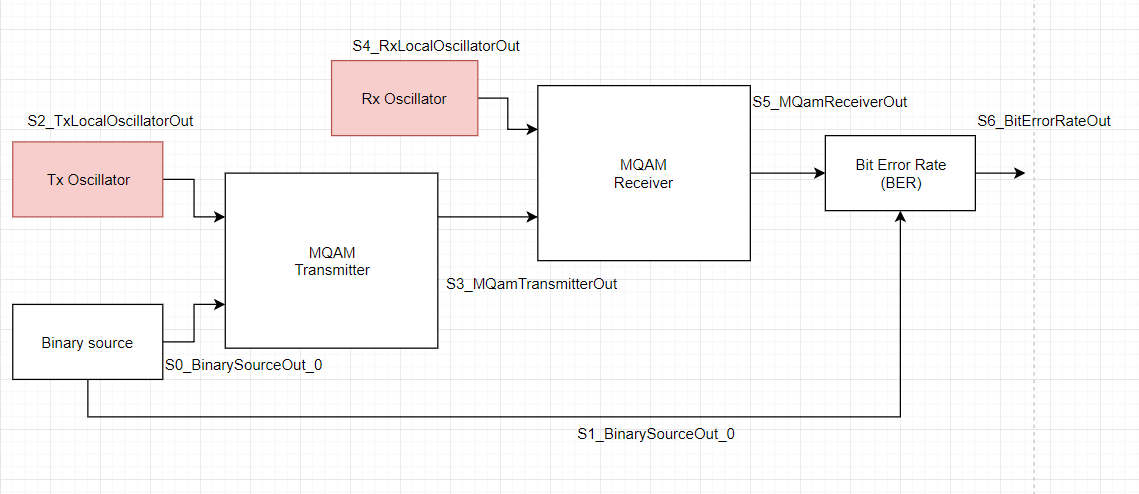
\includegraphics[scale=0.75]{../lib/m_qam_receiver/figure_PLoureiro/Diagrama_Blocos.png}
	\caption{Block diagram of a transmission system}\label{fig:homodyneRx_simple}
\end{figure}

\subsection*{Functional description}

This block accepts two optical inputs signals and outputs one binary signal that
corresponds to the decoded information transmitted in the input signal. It is a
complex
block (as it can be seen from figure \ref{fig:homodyneRx_blocks}) made up of
several simpler blocks whose description can be found in the
\textit{lib} repository.

\begin{figure}[H]
	\centering
	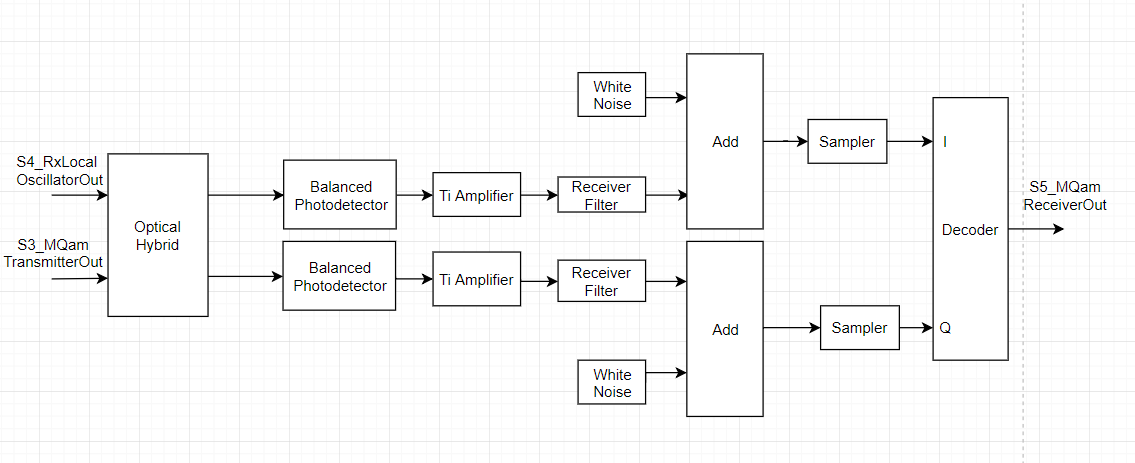
\includegraphics[width=\textwidth]{../lib/m_qam_receiver/figure_PLoureiro/Receiver.png}
	\caption{Schematic representation of the block homodyne
	receiver.}\label{fig:homodyneRx_blocks}
\end{figure}

\subsection*{Input parameters}

This block input parameters that can be manipulated by the user in
order to change the configuration of the receiver. Each parameter is changed by
calling a
particular function. In the following table
(Table~\ref{table}) the input parameters are
summarized.
%
\begin{table}[H]
	\begin{tabular}{|c|c|c|c|cccc}
		\cline{1-4}
		\textbf{Parameter} & \textbf{Type} & \textbf{Values} &   \textbf{Default}& \\ \cline{1-4}
        signalsFolderName & string & any & signals/\\
        & & & SuperBlock\_MQamReceiver \\ \cline{1-4}
        logValue & bool & any & true \\ \cline{1-4}
        logFileName & string & any & SuperBlock\_\\
        & & & \_MQamReceiver.txt \\ \cline{1-4}
		\multicolumn{4}{|c|}{ \textbf{Photodiodes} } \\ \cline{1-4}
		Responsivity & t\_real & any & 1\\ \cline{1-4}
		\multicolumn{4}{|c|}{ \textbf{TI Amplifier} } \\ \cline{1-4}
		NoiseSpectralDensity & t\_real & any & 1.5*10$^{-17}$ \\ \cline{1-4}
        gain & t\_real & any & 1*10$^4$ \\ \cline{1-4}
        fType & Filter & any$^1$ & LowPass \\ \cline{1-4}
        ctfFreq & double & any & 5 \\ \cline{1-4}
        irl & int & any & 128 \\ \cline{1-4}
        ir & vector$<$t\_real$>$ & any & 0 \\ \cline{1-4}
        fName & string & any & impulse\_response.imp \\ \cline{1-4}
        sBeginningOf & bool & any & true \\
        ImpulseResponse & & & \\ \cline{1-4}
		\multicolumn{4}{|c|}{ \textbf{General Noise} } \\ \cline{1-4}
		SamplingPeriod & t\_real & any & 1.0 \\ \cline{1-4}
        nSymbolPeriod   & t\_real & any & 1.0 \\ \cline{1-4}
        \multicolumn{4}{|c|}{ \textbf{Thermal noise} } \\ \cline{1-4}
        NoiseSpectralDensity & t\_real & any & 1.5*10$^{-17}$ \\ \cline{1-4}
        cp & bool & any & 0 \\ \cline{1-4}
        noiseSeeds & array$<$int, 2$>$ & any & 1 \\ \cline{1-4}
        seedType & SeedType & any$^2$ & RandomDevice \\ \cline{1-4}
        \multicolumn{4}{|c|}{ \textbf{Pulse shaper} } \\ \cline{1-4}
        impResponse & int & any & 16 \\
        TimeLength & & & \\ \cline{1-4}
        fType   & pulse\_shapper\_filter\_type & any$^3$ & RaisedCosine \\ \cline{1-4}
        rOffFactor & double & $\in \left[0,1\right]$ & 0.9 \\ \cline{1-4}
        ne & bool & any & false \\ \cline{1-4}
        pFilterMode & bool & any & false \\ \cline{1-4}
        sBeginningOf & bool & any & true \\
        ImpulseResponse & & & \\ \cline{1-4}
        \multicolumn{4}{|c|}{ \textbf{Sampler} } \\ \cline{1-4}
        sToSkip & int & any & 0 \\ \cline{1-4}
        \multicolumn{4}{|c|}{ \textbf{Decoder} } \\ \cline{1-4}
        iqAmplitudesValues & vector$<$t\_iqValues$>$ & any & \{ \{ 1, 1 \},\{ -1, 1 \}, \\
        &&&\{ -1, -1 \},\{ 1, -1 \} \} \\ \cline{1-4}
	\end{tabular}
	\caption{Binary source input parameters}
	\label{table}
\end{table}
$^1$ LowPass, Defined, Unitary \par
$^2$ RandomDevice, DefaultDeterministic, SingleSelected \par
$^3$ RaisedCosine, Gaussian, Square, RootRaisedCosine \par

\subsection*{Methods}

\begin{enumerate}
         \item Block Declaration and Initialization
             \begin{itemize}
                 \item MQamReceiver(initializer\_list$<$Signal *$>$ \&inputSig, initializer\_list$<$Signal *$>$ \&outputSig)
                 \item void initialize(void)
	             \item bool runBlock(void)
             \end{itemize}
         \item Functions to set parameters
             \begin{itemize}
                \item void setPhotodiodesResponsivity(t\_real Responsivity)
                \item void setGain(t\_real gain)
                \item void setAmplifierInputNoisePowerSpectralDensity(t\_real NoiseSpectralDensity)
                \item void setTiAmplifierFilterType(Filter fType)
                \item void setTiAmplifierCutoffFrequency(double ctfFreq)
                \item void setTiAmplifierImpulseResponseTimeLength\_symbolPeriods(int irl)
                \item void setElectricalFilterImpulseResponse(vector$<$t\_real$>$ ir)
                \item void setElectricalImpulseResponseFilename(string fName)
                \item void setElectricalSeeBeginningOfImpulseResponse\newline(bool sBeginningOfImpulseResponse)
                \item void setNoiseSamplingPeriod(t\_real SamplingPeriod)
                \item void setNoiseSymbolPeriod(t\_real nSymbolPeriod)
                \item void setThermalNoiseSpectralDensity(t\_real NoiseSpectralDensity)
                \item void setThermalNoisePower(t\_real NoiseSpectralDensity)
                \item void setThermalConstantPower(bool cp)
                \item void setSeeds(array$<$int, 2$>$ noiseSeeds)
                \item void setSeedType(SeedType seedType)
                \item void setThermalConstantPower(bool cp)
                \item void setImpulseResponseTimeLength(int impResponseTimeLength)
                \item void setFilterType(pulse\_shapper\_filter\_type fType)
                \item void setRollOffFactor(double rOffFactor)
                \item void usePassiveFilterMode(bool pFilterMode)
                \item void setRrcNormalizeEnergy(bool ne)
                \item void setMFImpulseResponseFilename(string fName)
                \item void setMFSeeBeginningOfImpulseResponse\newline(bool sBeginningOfImpulseResponse)
                \item void setSamplesToSkip(int sToSkip)
                \item void setIqAmplitudes(vector$<$t\_iqValues$>$ iqAmplitudesValues)
             \end{itemize}
         \item Functions to get parameters
             \begin{itemize}
                \item t\_real getGain(void)
                \item t\_real getAmplifierInputNoisePowerSpectralDensity(void)
                \item double const getElectricalSeeBeginningOfImpulseResponse(void)S
                \item double const getMFSeeBeginningOfImpulseResponse(void)
                \item vector$<$t\_iqValues$>$ const getIqAmplitudes(void)
             \end{itemize}
     \end{enumerate}

\subsection*{Input Signals}

\subparagraph*{Number:} 2

\subparagraph*{Type:} One optical signal from the local oscillator - S4\_RxLocalOscillatorOut \par One optical signal from the transmitter - S3\_MQamTransmitterOut

\subsection*{Output Signals}

\subparagraph*{Number:} 1

\subparagraph*{Type:} One Binary signal - S5\_MQamReceiverOut

\newpage
\subsection*{Example}
\subsubsection*{Receiver sensitivity}

In order to analyze the sensitivity of the receiver were tested some thermal noise power values to obtain to obtain the respective BER. The graph is shown in figure \ref{Thermal_BER}.

\begin{figure}[H]
	\centering
	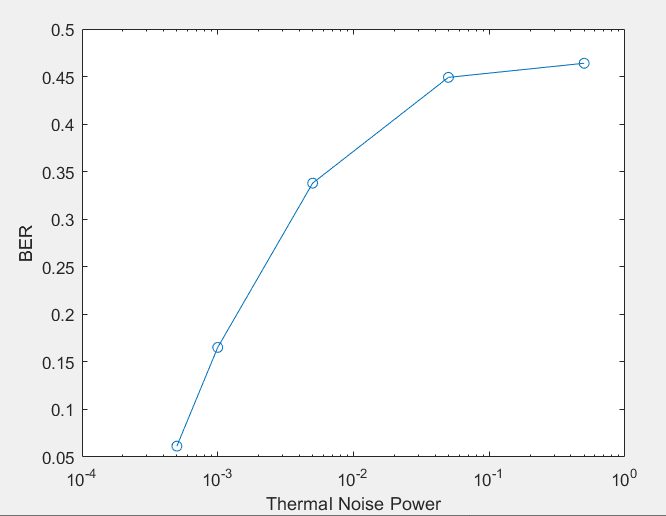
\includegraphics[width=0.6\textwidth]{./lib/m_qam_receiver/figure_PLoureiro/Thermal_BER.png}
	\caption{Example of the BER in function of Thermal noise power }\label{Thermal_BER}
\end{figure}

As expected the increase of the thermal noise power increase also the BER.

\subsubsection*{Impact of the electrical amplifier}
To evaluate the impact of the electrical amplifier, it was tried to change the bandwidth of the filter. The signals at the output of the electrical amplifier was compared when the bandwidth was 50Ghz and 5GHz.

\begin{figure}[H]
	\centering
        \begin{subfigure}{.55\textwidth}
        \centering
        	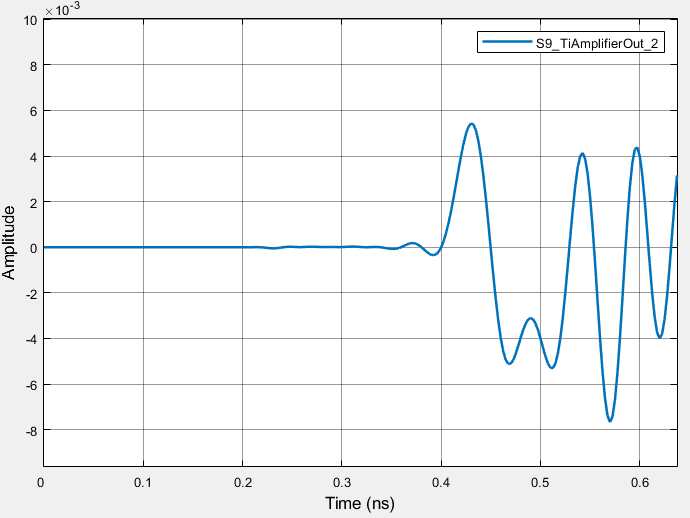
\includegraphics[scale=0.45]{./lib/m_qam_receiver/figure_PLoureiro/4QAM_ElectricalNoise_50e9_time.png}
        \label{Example_Time_50GHz}\caption{Time domain when the bandwidth was 5GHz}
        \end{subfigure}%
        \begin{subfigure}{.55\textwidth}
        \centering
        	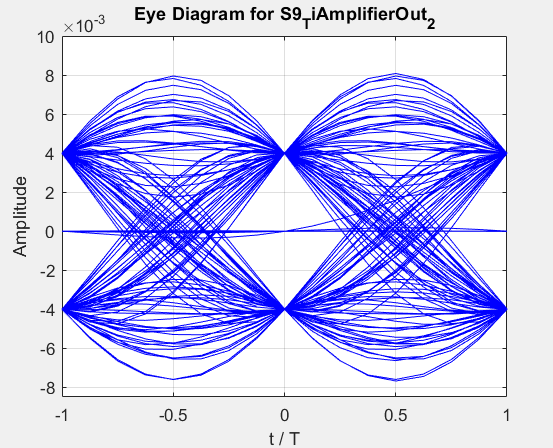
\includegraphics[scale=0.45]{./lib/m_qam_receiver/figure_PLoureiro/4QAM_ElectricalNoise_50e9_Eye.png}
        	\caption{Eye diagram when the bandwidth was 50GHz}\label{Example_Eye_50GHz}
        \end{subfigure}
        \caption{}\label{50GHz}
\end{figure}

\begin{figure}[H]
	\centering
        \begin{subfigure}{.55\textwidth}
        \centering
        	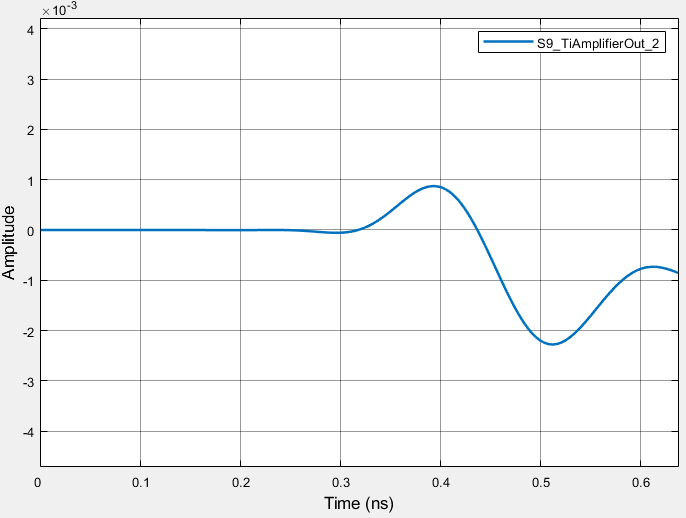
\includegraphics[scale=0.45]{./lib/m_qam_receiver/figure_PLoureiro/4QAM_ElectricallNoise_50e8_time.png}
        \label{Example_Time_5GHz}\caption{Time domain when the bandwidth was 5GHz}
        \end{subfigure}%
        \begin{subfigure}{.55\textwidth}
        \centering
        	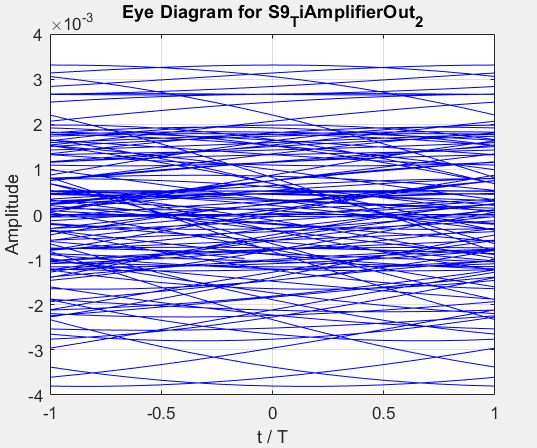
\includegraphics[scale=0.45]{./lib/m_qam_receiver/figure_PLoureiro/4QAM_ElectricalNoise_50e8_Eye.png}
        	\caption{Eye diagram when the bandwidth was 5GHz}\label{Example_Eye_5GHz}
        \end{subfigure}
        \caption{}\label{5GHz}
\end{figure}

By the figures \ref{5GHz} and \ref{50GHz} when the bandwidth was reduced from 50GHz to 5GHz the signal was distorted and BER increased.\par

Also was tested the impact of the gain. To analyze this, was used the Thermal Noise Power of 5*10$^{-1}$ and was changed the gain between 1 and 10.
\begin{equation*}
BER_{Gain1} = 0.463983
\end{equation*}
\begin{equation*}
BER_{Gain10} = 0.308263
\end{equation*}
If the gain is 10 times greater the influence of the noise is 10 times lower, so the BER decreased with the increased of the gain.

\subsection*{Open Issues}
When was tested the impact of the local oscillator power (increase the power), wasn't observed any influence of the quantum noise.
